\chapter{Discusión}\label{discusion}

\subsection{Metodología de trabajo}

En todo proyecto no solo es importante el resultado, sino el camino que lleva a éste último. Durante el desarrollo del proyecto se utilizó la metodología ágil SCRUM, la cual consta a grandes rasgos de una pila Backlog de requerimientos, Sprints correspondientes a intervalos acotados de trabajos destinados a cumplir una cierta porción de los requerimientos y reuniones bastante más consecutivas que con otras metodologías. 

Para las especificaciones del proyecto se hizo bastante cómodo su uso, pues grandes cambios suponían solo modificar ciertos Sprint y en caso de encontrar problemas o bloqueantes, por la comunicación frecuente dentro del equipo se podían tomar decisiones en un corto periodo de tiempo.

\begin{figure}[H]
	\centering
	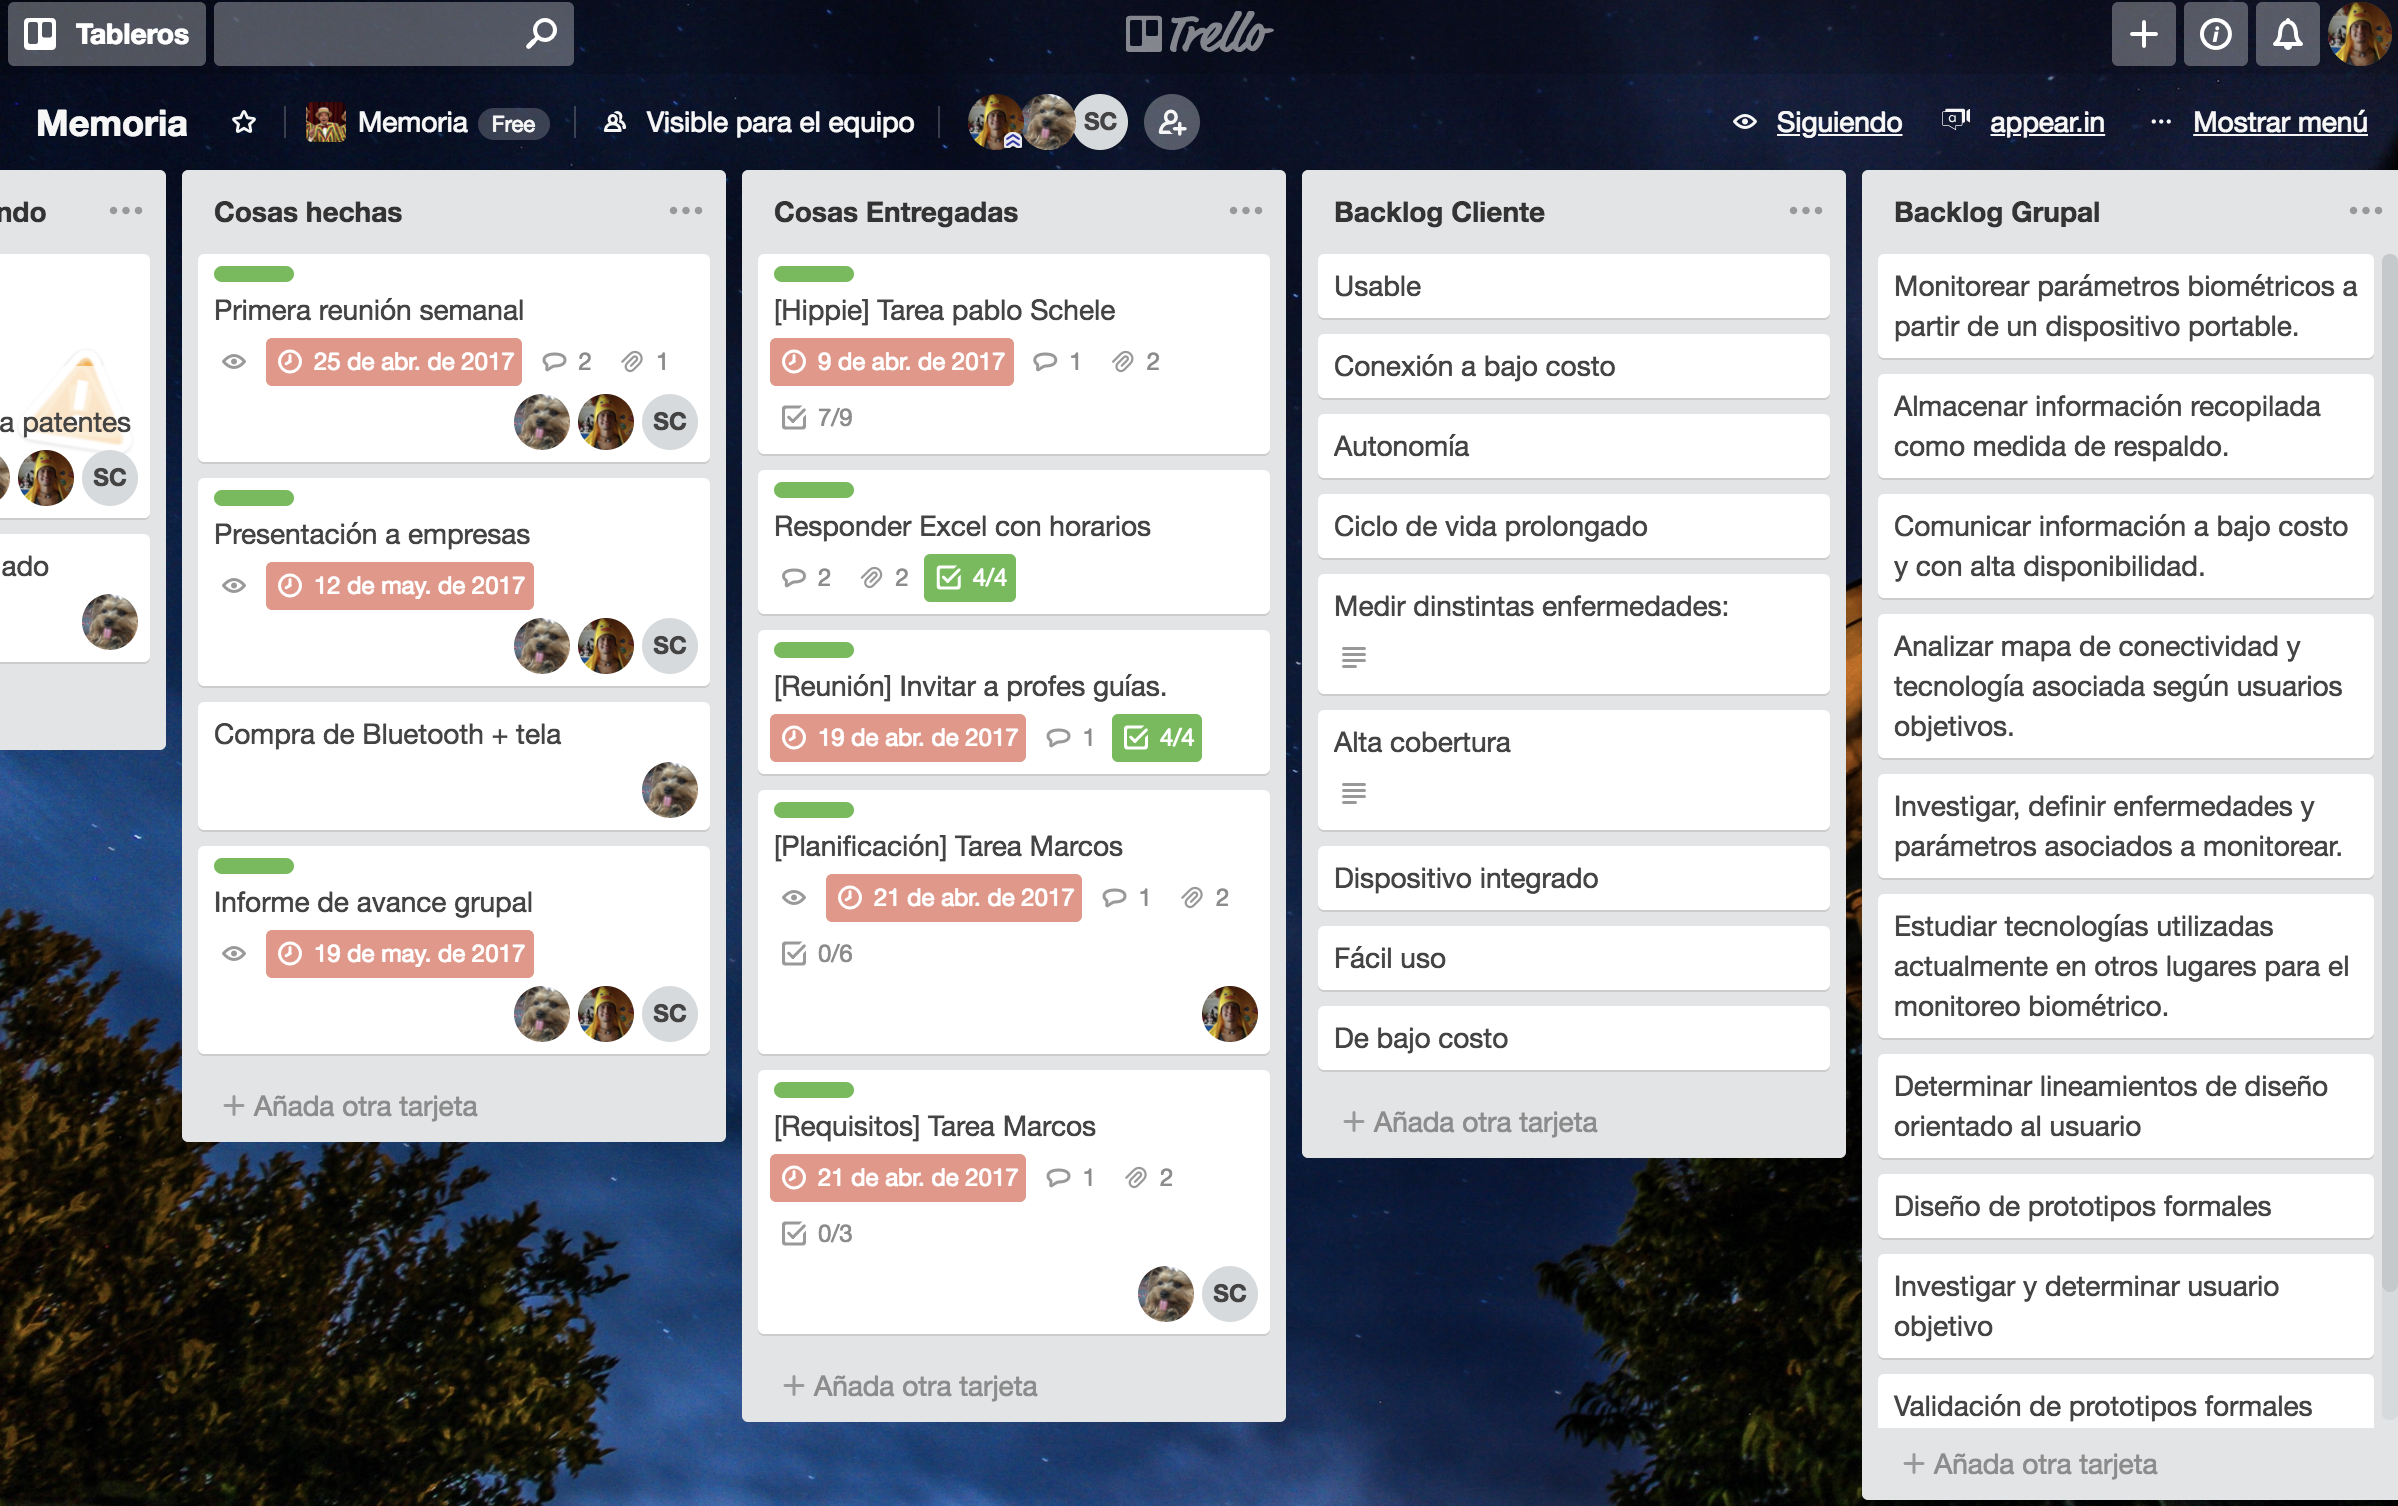
\includegraphics[scale=0.3]{figuras/discusion/trello.png}
	\caption{Tableros empleados en Trello}
	\label{trello}
\end{figure}


Para llevar a cabo la organización se hizo uso de Trello, una plataforma de organización laboral común, en tiempo real y basada en la nube, la cual permite el seguimiento de los distintos avances y trabajos de cada uno de los integrantes del equipo. Como se puede observar en la figura \ref{trello} es posible trabajar en base a tableros, listas y tarjetas (uno contenedor de otro respectivamente).


\subsection{Relaciones públicas}

Durante el transcurso del proyecto se hizo patente la necesidad de contactar con actores reales que enfrentaran problemáticas asociadas. Por este motivo, se realizaron contactos con distintos profesionales en búsqueda de información y/o alianzas:

\textbf{Proyecto Almohadita}: Proyecto de monitoreo y clasificación de riesgo intrahospitalario a distancia. Implementado en el hospital Dr. Exequiel González Cortés y a cargo de Sebastián Ríos, Investigador ISCI (Instituto de Sistemas Complejos de Ingeniería) Académico FCFM (Facultad de Ciencias Físicas y Matemáticas) U Chile. 

No se logró establecer una reunión formal con el equipo desarrollador de este proyecto, su relevancia yacía en la cercanía con los objetivos entre los proyectos (monitoreo a distancia).

\textbf{SubTel}: En un unicio se estableció contacto con la Subsecretaría de Telecomunicaciones con el fin de obtener información de cobertura nacional de las distintas bandas celulares disponibles. 

Dando como resultado la ley de Neutralidad de la red, respuesta adjunta en los anexos.

\textbf{Profesionales de la Salud}: Se contactó con la enfermera jefa de urgencias Elizabeth Nievas, y los doctores Fabián Álvarez (Jefe de Urgencias) y Cristian Mondaca (Jefe del programa salud cardiovascular y jefe de farmacia). Todos del hospital de Quintero Adriana Cousiño, con los cuales se contrastaron requerimientos y se barajó la factibilidad de realizar pruebas con pacientes.

La información recopilada permitió un lineamiento más cercano del proyecto a la realidad (cantidad de derivaciones necesarias, entre otros).

\newpage

\textbf{DesafIoT (3IE)}: Durante el verano de 2018, se fue partícipe como equipo multidisciplinario del desafío propuesto por la incubadora de la Universidad Federico Santa María 3IE. El cual estaba destinado a equipos con desarrollos de proyectos con tecnología IoT (Internet of Things). 

No fue posible pasar de la primera selección, principalmente por aspectos económicos del proyecto (poca viabilidad por falta de clientes actuales e interesados) y del poco interés generado hacia los jueces de la propuesta (falta de innovación).

\subsection{Trabajos futuros}



\subsection{Nuevas tecnologías y su impacto en el proyecto}

